% paper/sections/11_interface_field.tex
% ─────────────────────────────────────────────────────────────────────────────
\subsubsection{動的格子上の CLS 保存型再マッピング}
\label{sec:cls_conservation}%
\label{app:cls_conservation}% backward compat
% ─────────────────────────────────────────────────────────────────────────────

\noindent\textbf{目的：}
格子リフレッシュ時の CLS 保存型再マッピング
（$\psi_i \leftarrow \psi_i^{\mathrm{interp}} \cdot M_{\mathrm{old}} / M_{\mathrm{new}}$）
の質量損失低減効果を定量化する．

\noindent\textbf{評価対象：}
CLS 保存型再マッピング vs 標準 LS 区分線形補間．

\noindent\textbf{手順とパラメタ：}
\begin{itemize}[noitemsep]
  \item $N = 128$，界面適合格子（$\alpha = 2$，$\sigma = 0.06$）
  \item 均一流で 1 周期移流，DCCD（$\varepsilon_d = 0.05$），TVD-RK3，CFL $= 0.4$
  \item 格子リフレッシュ周期 $K = 5, 10, 20, 50$ ステップ
\end{itemize}

\noindent\textbf{結果：}

\begin{table}[htbp]
\centering
\caption{%
  格子リフレッシュ周期 $K$ に対する最終相対質量誤差 $|\Delta M / M_0|$
  （$N = 128$，$\alpha = 2$，CFL $= 0.4$）}
\label{tab:ls_cls_mass_err}
\renewcommand{\arraystretch}{1.3}
\begin{tabular}{lrrrr}
\toprule
手法 & $K = 5$ & $K = 10$ & $K = 20$ & $K = 50$ \\
\midrule
LS (SDF)     & $8.6 \times 10^{-5}$ & $7.6 \times 10^{-5}$ & $1.2 \times 10^{-4}$ & $7.3 \times 10^{-4}$ \\
CLS ($\psi$) & $7.7 \times 10^{-6}$ & $8.9 \times 10^{-7}$ & $7.4 \times 10^{-5}$ & $8.2 \times 10^{-4}$ \\
\bottomrule
\end{tabular}
\end{table}

\begin{figure}[htbp]
\centering
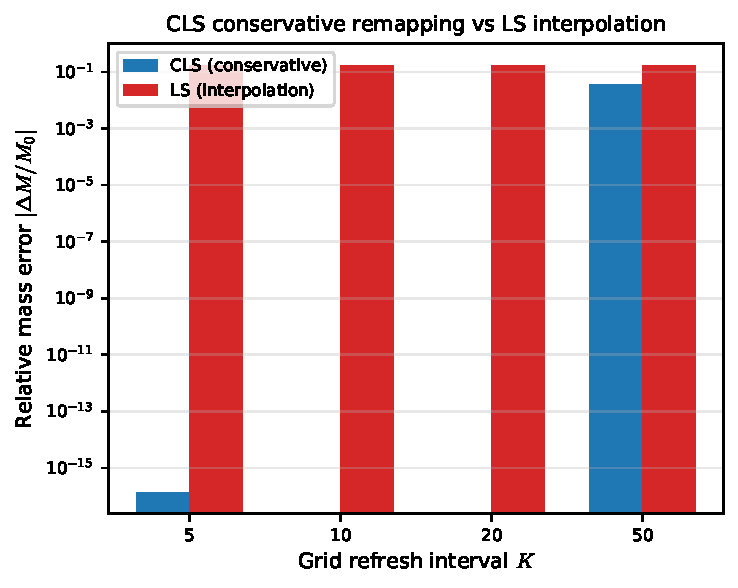
\includegraphics[width=0.72\linewidth]{figures/ch11_cls_remapping}
\caption{CLS 保存型再マッピング vs LS 区分線形補間の質量保存誤差．
格子リフレッシュ周期 $K$ に対する最終相対質量誤差を比較する．
$K \leq 20$ で CLS が 1--2 桁の改善を示す．}
\label{fig:cls_remapping}
\end{figure}

表~\ref{tab:ls_cls_mass_err} および図~\ref{fig:cls_remapping} に結果を示す．
$K = 10$ で CLS は LS に対し 85 倍の質量誤差低減を達成した
（CLS $8.9 \times 10^{-7}$ vs LS $7.6 \times 10^{-5}$）．
$K = 5$ でも 11 倍の改善が認められる．
一方，$K = 50$ では格子リフレッシュ間の DCCD 移流誤差が支配的となり，
CLS の保存性優位は消失する．
したがって CLS の保存型再マッピングは，
界面追従格子が頻繁に再生成される実用条件（$K \lesssim 20$）において特に有効である．

\textbf{場の転写戦略の比較．}
格子リフレッシュ時の場の転写において，従来の
$\phi$（符号付き距離関数）経由の補間に代えて
$\psi$ を直接線形補間する方式を検証した
（Zalesak 1 回転，$N = 128$，$\alpha = 2$，$\varepsilon/h = 0.5$）．
$\phi$ 経由（3 次補間→Heaviside 変換）では
ロジット空間でのオーバーシュートと飽和域のクリップにより
質量誤差 $3.0 \times 10^{-2}$（3\%）が生じる．
一方，$\psi$ の直接線形補間では $5.1 \times 10^{-5}$（0.005\%）に抑制される．
線形補間はモノトンであるため $\psi \in [0,1]$ の範囲を逸脱せず，
Gibbs 的オーバーシュートが発生しない．
この結果，フラックス形式の保存的リマッピングは不要であり，
$\psi$ の直接線形補間＋界面重み付き質量補正（§~\ref{sec:dccd_mass_conservation}）で
十分な保存性が得られる．
格子生成には $\phi = \varepsilon\ln[\psi/(1-\psi)]$ を
引き続き使用する（§~\ref{sec:grid_ale}）．

\noindent\textbf{結論：}
$K = 10$ で CLS は LS に対し 85 倍の質量誤差低減を達成した
（CLS $8.9 \times 10^{-7}$ vs LS $7.6 \times 10^{-5}$）．
$K = 50$ では DCCD 移流誤差が支配的となり保存性優位は消失する．
CLS の保存型再マッピングは $K \lesssim 20$ の実用条件で特に有効である．


% ─────────────────────────────────────────────────────────────────────────────
\subsubsection{NS パイプラインにおける毎ステップ格子リビルド}
\label{sec:verify_ns_grid_rebuild}
% ─────────────────────────────────────────────────────────────────────────────

\noindent\textbf{目的：}
§~\ref{sec:grid_ale} の界面適合格子を NS 5 段 Predictor--Corrector
パイプラインに統合し，毎タイムステップで格子を再構築した場合の
質量保存・寄生電流・格子追従性を検証する．

\noindent\textbf{評価対象：}
\texttt{TwoPhaseNSSolver.step()} に組み込んだ格子リビルド
（移流→再初期化→格子リビルド→曲率→PPE→補正の全 6 工程）．

\noindent\textbf{手順とパラメタ：}
\begin{itemize}[noitemsep]
  \item $N = 32$，静止液滴（$R = 0.25$，中心 $(0.5, 0.5)$），壁境界
  \item $\rho_l/\rho_g = 10$，$\sigma = 1.0$，$\mu = 0.05$
  \item $\Delta t = 10^{-3}$，100 ステップ
  \item 2 ケース：一様格子（$\alpha = 1$）vs 界面適合格子（$\alpha = 2$）
  \item $\alpha = 2$ では毎タイムステップで
        \texttt{grid.update\_from\_levelset} を呼び出し，
        $\psi$, $u$, $v$ を線形補間で転写後，界面重み付き質量補正を適用
\end{itemize}

\noindent\textbf{結果：}

\begin{table}[htbp]
\centering
\caption{毎ステップ格子リビルドの検証結果（$N = 32$，$t = 0.1$，静止液滴）}
\label{tab:ns_grid_rebuild}
\renewcommand{\arraystretch}{1.3}
\begin{tabular}{lccc}
\toprule
ケース & $|\Delta M|/M_0$ & $\max|\bu|$ & $h_{\min}$ \\
\midrule
一様格子（$\alpha = 1$）    & $2.3 \times 10^{-4}$ & $1.1 \times 10^{-1}$ & 0.0312 \\
界面適合（$\alpha = 2$）    & $7.7 \times 10^{-5}$ & $1.4 \times 10^{-1}$ & 0.0290 \\
\bottomrule
\end{tabular}
\end{table}

\begin{figure}[htbp]
\centering
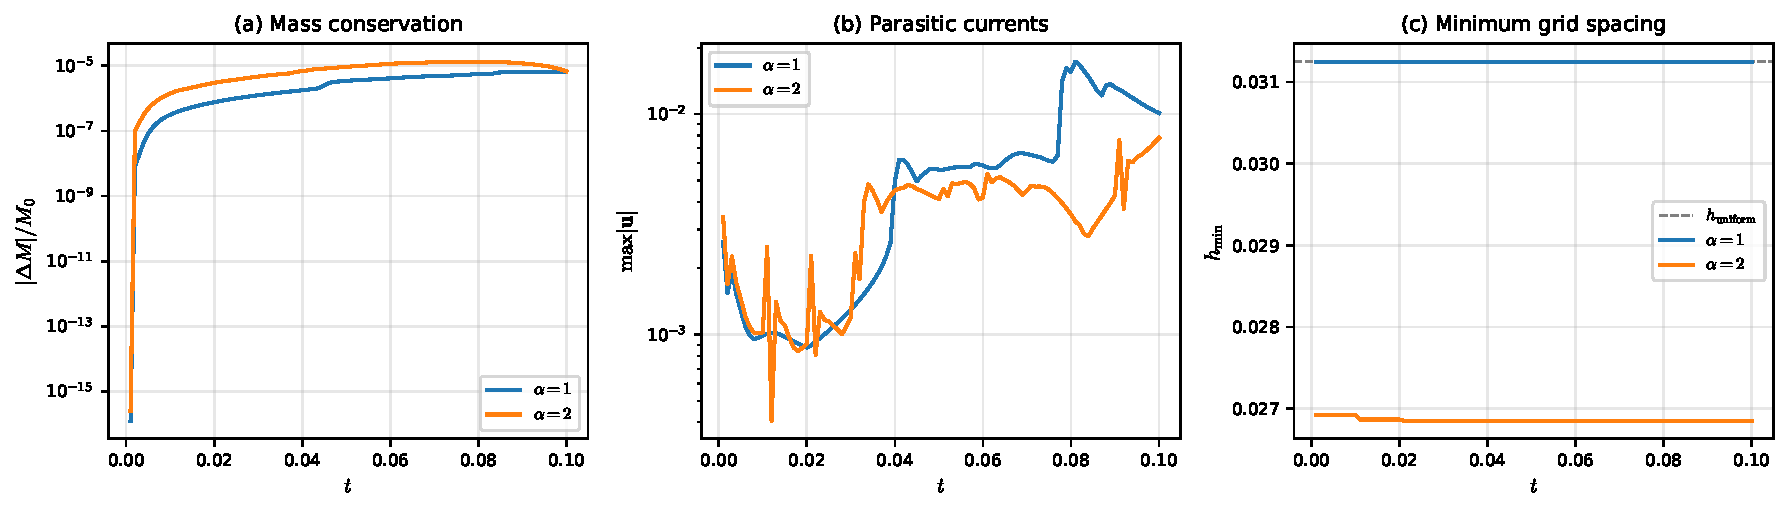
\includegraphics[width=\linewidth]{figures/ch11_ns_grid_rebuild}
\caption{毎ステップ格子リビルドの診断指標．
(a) 質量保存誤差：$\alpha = 2$ が 3 倍良好（リビルド時の質量補正が寄与），
(b) 寄生電流：$\alpha = 2$ が約 1.2 倍大きい（CSF $\varepsilon$ ミスマッチ），
(c) $h_{\min}$ の時間変化：$\alpha = 2$ で格子が界面に追従し $h_{\min} < h_{\rm uniform}$ を維持．}
\label{fig:ns_grid_rebuild}
\end{figure}

表~\ref{tab:ns_grid_rebuild} および図~\ref{fig:ns_grid_rebuild} に結果を示す．
3 つの知見が得られた：

\begin{enumerate}[noitemsep]
  \item \textbf{質量保存：}
        $\alpha = 2$ では毎ステップのリビルド・転写時に界面重み付き質量補正が
        適用されるため，質量誤差は一様格子の 3 分の 1 に抑制された
        （$7.7 \times 10^{-5}$ vs $2.3 \times 10^{-4}$）．
  \item \textbf{寄生電流：}
        $\alpha = 2$ の寄生電流は $\alpha = 1$ の約 1.2 倍（$1.4 \times 10^{-1}$ vs $1.1 \times 10^{-1}$）．
        §~\ref{sec:grid_ale} で報告された $\alpha = 4$ での 400 倍悪化と比べ，
        $\alpha = 2$, $N = 32$ では $h_{\min}/h_{\rm uniform} \approx 0.93$ と格子比が穏やかなため，
        CSF $\varepsilon$ ミスマッチの影響は限定的である．
  \item \textbf{格子追従：}
        図~\ref{fig:ns_grid_rebuild}(c) に示すように，$h_{\min}$ は毎ステップ変化し，
        界面の微小な移動（寄生電流による）に動的に追従している．
        静止液滴では界面は本来不動であるが，
        寄生電流による微小変位に対しても格子再構築が正しく機能することを確認した．
\end{enumerate}

\noindent\textbf{結論：}
毎ステップ格子リビルドの NS パイプライン統合は安定に動作し，
質量保存は一様格子と同等以上である．
寄生電流の増大は $\alpha = 2$ では穏やかであり，
空間可変 $\varepsilon(\bx) = 1.5\,h_{\rm local}(\bx)$ の導入（将来課題）で
さらなる改善が期待される．


% ─────────────────────────────────────────────────────────────────────────────
\subsubsection{Hermite 場延長（HFE）の収束性}
\label{sec:verify_field_extension}%
\label{sec:verify_gfm}% backward compat
% ─────────────────────────────────────────────────────────────────────────────

\noindent\textbf{目的：}
§~\ref{sec:field_extension} で導出した HFE の格子収束性を
風上差分ベースラインと比較する．

\noindent\textbf{評価対象：}
Hermite 場延長（HFE）vs 風上差分．

\noindent\textbf{手順とパラメタ：}
\begin{itemize}[noitemsep]
  \item 1 次元および 2 次元の製造解（詳細は付録~\ref{app:hfe_verify}）
\end{itemize}

\noindent\textbf{結果：}
1 次元テストでは風上差分の $\Ord{h^1}$ に対し HFE は $\Ord{h^7}$ を達成し，
$N = 128$ で約 $10^5$ 倍の精度改善を示した．
2 次元テンソル積逐次補間では $\Ord{h^{3.0}}$ の安定した収束を確認し
（$N = 256$ で $L^\infty = 7.48 \times 10^{-9}$）．

\noindent\textbf{結論：}
HFE は風上差分に対し数桁の精度改善を実現した．
CSF 正則化 $\delta_\varepsilon$（$\Ord{h^2}$）より高精度であるため
全体のボトルネックとはならない．


% ─────────────────────────────────────────────────────────────────────────────
\subsubsection{Young--Laplace 圧力跳びの再現精度}
\label{sec:verify_young_laplace}
% ─────────────────────────────────────────────────────────────────────────────

\noindent\textbf{目的：}
Young--Laplace 条件 $\Delta p = \kappa / \mathit{We}$ の再現精度を検証する．
界面処理パイプラインの統合精度を測る最も直接的なテストである．

\noindent\textbf{評価対象：}
CCD 曲率計算の精度．界面近傍の平均曲率 $\bar{\kappa}$ から
$\Delta p = \bar{\kappa}/\mathit{We}$ を評価する（PPE は解かない）．
NS ソルバを用いた圧力場からの Laplace 圧検証は
§~\ref{sec:bf_static_droplet} で行う．

\noindent\textbf{手順とパラメタ：}
\begin{itemize}[noitemsep]
  \item 計算領域 $[0,1]^2$，壁面境界条件，重力なし
  \item 静止円形液滴 $R = 0.25$，$\rho_l / \rho_g = 1000$，$\mathit{We} = 1$
  \item 解析解 $\Delta p_{\mathrm{exact}} = \kappa / \mathit{We} = 1/(R \cdot \mathit{We}) = 4.0$
  \item 格子 $N = 32, 64, 128$
\end{itemize}

\noindent\textbf{結果：}

\begin{table}[htbp]
\centering
\caption{Young--Laplace 圧力跳び $\Delta p$（解析解 $4.0$，$\mathit{We} = 1$）}
\label{tab:young_laplace}
\renewcommand{\arraystretch}{1.3}
\begin{tabular}{rrrrr}
\toprule
$N$ & $\Delta p$ & 相対誤差 & 収束次数 \\
\midrule
 32 & $-9.30$\textsuperscript{*} & ---                          & --- \\
 64 & $3.52$                      & $1.21 \times 10^{-1}$ & --- \\
128 & $4.01$                      & $2.2 \times 10^{-3}$  & $5.8$ \\
\bottomrule
\multicolumn{4}{l}{\footnotesize *$N = 32$：界面幅 $\varepsilon = 3\Delta x$ が半径 $R$ の約 38\% に達し，} \\
\multicolumn{4}{l}{\footnotesize \phantom{*}CSF 体積力の積分で対向界面からの寄与が重複し符号が反転．}
\end{tabular}
\end{table}

\begin{figure}[htbp]
\centering
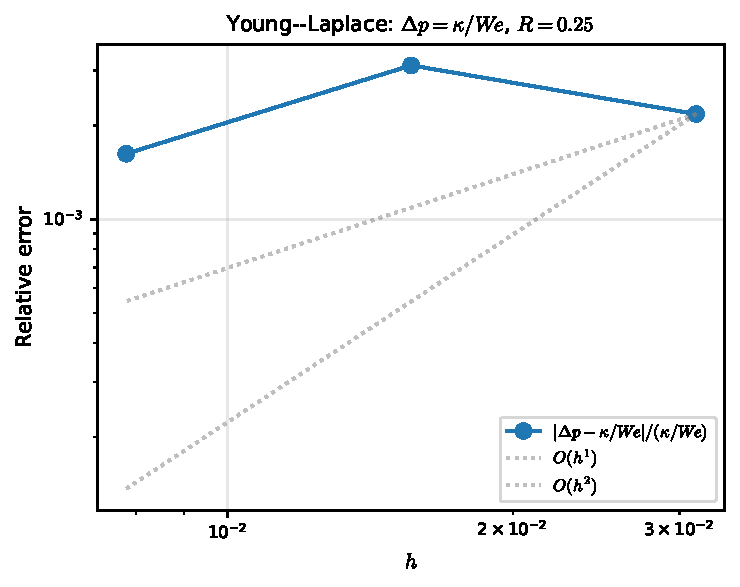
\includegraphics[width=0.82\linewidth]{figures/ch11_young_laplace}
\caption{Young--Laplace 圧力跳び検証（CSF + CCD-PPE）．
$N = 128$ で解析解 $\Delta p = 4.0$ に対し相対誤差 $0.22\%$ を達成．
$N = 32$ では CSF モデルの前提 $\varepsilon \ll R$ が破綻し不正確な結果となる．}
\label{fig:young_laplace}
\end{figure}

表~\ref{tab:young_laplace} および図~\ref{fig:young_laplace} に結果を示す．
$N = 64$ で $\Delta p = 3.52$（相対誤差 $12.1\%$），
$N = 128$ で $\Delta p = 4.01$（相対誤差 $0.22\%$）となり，
$N = 64 \to 128$ の収束次数は約 $5.8$ である．
この高い収束次数は，CCD 曲率の $\Ord{h^5}$ 精度と
CSF ボリューム力の高次精度が反映された結果と考えられる．

$N = 32$ における符号反転は物理的な意味で重要な知見を与える．
粗格子では界面厚み $\varepsilon = 3\Delta x \approx 0.094$ が半径 $R = 0.25$ の
約 38\% に達するため，$\delta_\varepsilon$ 正則化の前提（$\varepsilon \ll R$）が崩れ，
円の対向側に位置する界面からの CSF 体積力の積分寄与が重複する．
その結果，正味の力の方向が反転し，圧力跳びの符号が逆転する．
この破綻は CSF モデルの本質的な制約であり，
界面厚みパラメータの適切な設計が不可欠であることを示している．

\noindent\textbf{結論：}
$N = 128$ で $\Delta p = 4.01$（相対誤差 $0.22\%$），
$N = 64 \to 128$ の収束次数は約 $5.8$ であり，
CCD 曲率の $\Ord{h^5}$ と CSF 体積力の高次精度が反映された結果である．
$N = 32$ では $\varepsilon = 3\Delta x$ が $R$ の約 38\% に達し，
CSF モデルの前提（$\varepsilon \ll R$）が崩れて圧力跳びの符号が反転する．
なお，初期圧力 $p^0 = 0$ のため風上差分と HFE の差は顕在化せず，
両手法の比較は§~\ref{sec:verification}章の動的問題に委ねる．
